\section{Eigengesichter} \label{sec:facespace}
\begin{tcolorbox}
	\centerline{\textbf{Lernziele Kapitel~\ref{sec:facespace}}}
	\begin{enumerate}[leftmargin=*,label=\thesection.\arabic*]
		\item Den Durchschnitt einer Familie von Vektoren geometrisch \textit{verstehen}.
		\item Die Translation von Punkten um einen Vektor geometrisch \textit{verstehen}.
		\item Die Begriffe Durchschnittsgesicht, Differenzgesicht und Eigengesicht \textit{erklären} können.
	\end{enumerate}
\end{tcolorbox}
Seien nun $M,N\in\mathbb N$ fix.
Wir haben im letzten Kapitel gesehen, wie man schwarz-weiss Bilder der Auflösung $M\times N$ als Vektoren in $\mathbb R^{M\cdot N}$ verstehen kann.
Die Bilder müssen dafür nicht unbedingt ein Gesicht zeigen.
Die Pixel können sogar völlig zufällige Graustufen aufweisen, so dass auf dem Bild nichts sinnvolles zu erkennen ist.
Dies führt uns zu folgender Beobachtung:
Nur die wenigsten Vektoren in $\mathbb R^{M\cdot N}$ entsprechen einem Gesicht.
Wir wollen uns näher mit dieser Beobachtung befassen.

Sei $K\in\mathbb N$ die Anzahl aller Bilder von allen Personen unserer Datenbank.
Jedes Bild soll dabei die Auflösung $M\times N$ haben.
Wir betrachten alle Bilder der Datenbank als Vektoren $\vec b_1,\ldots,\vec b_K\in\mathbb R^{M\cdot N}$.
Diese Darstellung erlaubt uns, das \textit{Durchschnittsgesicht}, wir nennen es $\vec m\in\mathbb R^{M\cdot N}$, zu definieren
\begin{equation*}
	\vec m=\frac{1}{K}\left(\vec b_1+\ldots+\vec b_K\right).
\end{equation*}
Das Durchschnittsgesicht lässt sich wieder als Bild ausgeben.
Aber wie sieht so ein Durchschnittsgesicht aus?
Das werden wir in folgender Übung herausfinden.
\begin{aufgabe}
	Ergänzen Sie im File \texttt{eigenfaces.py} die Funktion \texttt{meanface(b\_list)}.
	Dabei ist \texttt{b\_list} die Liste der Länge $K$ der Vektoren $\vec b_1,\ldots,\vec b_K$.
	Der Rückgabewert soll das Durchschnittsgesicht $\vec m$ sein.
	Sie können die ihre Lösung überprüfen indem Sie das Skript \texttt{meanface\_test.py} laufen lassen.
	\textit{Hinweis:} Die Python Funktionen \texttt{len(...) und sum(...)} können nützlich sein.
\end{aufgabe}
\begin{losung*}
	Hier ist eine mögliche Lösung und das davon mit \texttt{meanface\_test.py} generierte Durchschnittsgesicht.\\[0.5cm]
	\begin{minipage}{0.45\textwidth}
\begin{lstlisting}[style=python]
def meanface(b_list):
	K = len(b_list)
	return sum(b_list) / K
\end{lstlisting}
	\end{minipage}\hfill
	\begin{minipage}{0.3\textwidth}\vspace{-1cm}
		\centering\hfill Durchschnittsgesicht:
	\end{minipage}
	\begin{minipage}{0.2\textwidth}\vspace{-1cm}
		\centering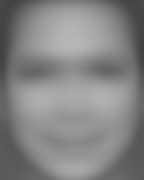
\includegraphics[width=0.6\textwidth]{images/facespace/meanface}
	\end{minipage}
\end{losung*}
Nachdem wir nun das Durchschnittsgesicht gebildet haben, berechnen wir nun die \textit{Differenzgesichter} $\vec a_1,\ldots,\vec a_K$.
Diese sind definiert als
\begin{equation*}
	\vec a_k=\vec b_k-\vec m,\quad k\in\left\{1,\ldots,K\right\}.
\end{equation*}
Die eben eingeführten Begriffe sind links in Abbildung~\ref{fig:meandiff} stark vereinfacht visualisiert.
\begin{figure}[ht]
	\centering
	\begin{minipage}{0.5\textwidth}
		\centering
		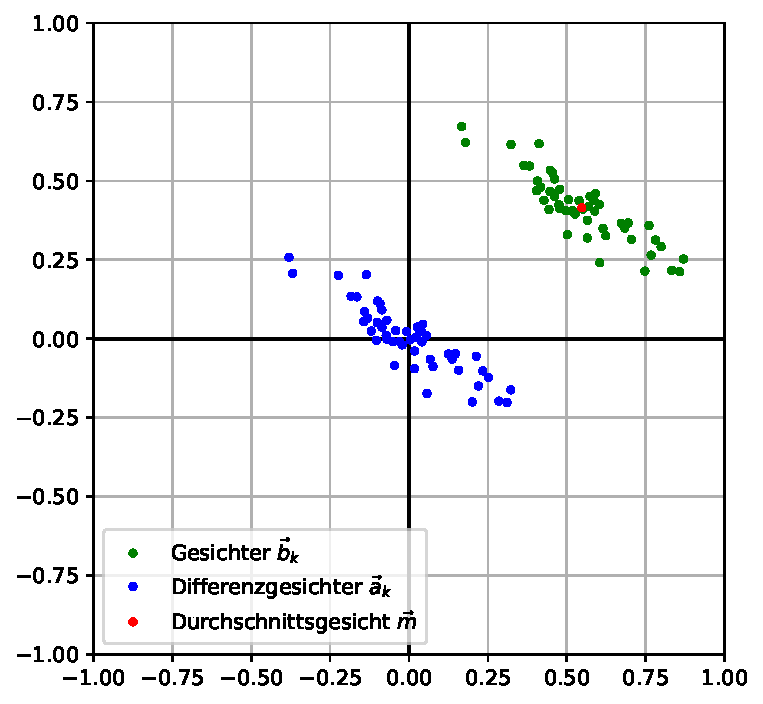
\includegraphics[width=\textwidth]{images/facespace/meandiff}
	\end{minipage}\hfill
	\begin{minipage}{0.5\textwidth}
		\centering
		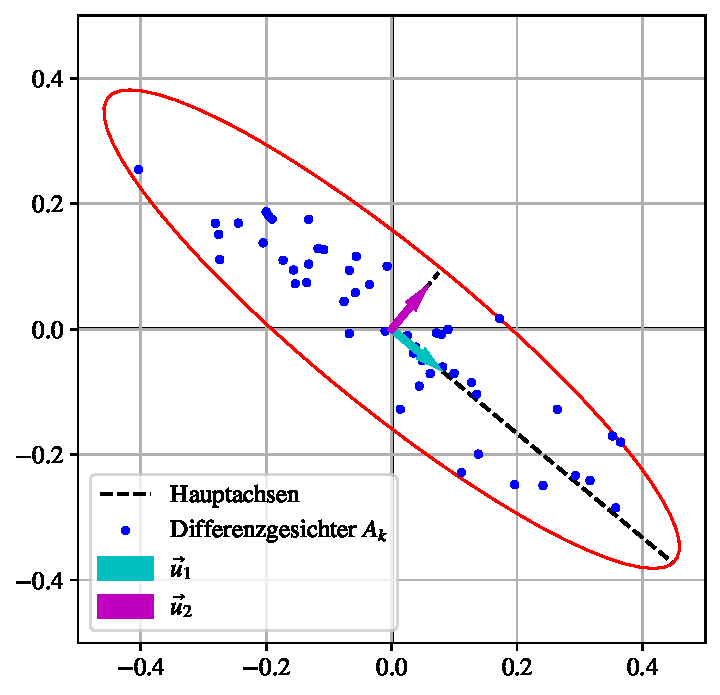
\includegraphics[width=\textwidth]{images/facespace/principal_components}
	\end{minipage}
	\caption{Die Gesichter werden um den Ursprung zentriert indem man das Durchschnittsgesicht subtrahiert (links).
	Die Eigengesichter sind die orthonormalen Vektoren entlang den Hauptachsen (rechts).}
	\label{fig:meandiff}
\end{figure}
\begin{aufgabe} \label{aufg:hmmc}
	Nennen Sie einen Unterschied und eine Gemeinsamkeit der vereinfachten Darstellung links in Abbildung~\ref{fig:meandiff} zu unserer tatsächlichen Situation mit Bildern von Gesichtern.
	Gehen Sie davon aus, dass unsere Bilder eine Auflösung von $M=180$ und $N=144$ haben, wie im letzten Kapitel.
\end{aufgabe}
\begin{losung*}
	Als Vektoren aufgefasst sind die Gesichter Punkte im $\mathbb R^{M\cdot N}$.
	Für $M=180$ und $N=144$ wären das Punkte im $\mathbb R^{25'920}$ und nicht im $\mathbb R^2$ wie in der Abbildung.
	Anders ausgedrückt zeigt die Abbildung den Spezialfall $M\cdot N=2$.
	Das entspricht Bilder die nur aus zwei Pixeln bestehen.
	Andererseits wird in der Abbildung korrekt gezeigt, dass die Komponenten der Gesichts-Vektoren $\vec b_k$ nur Werte zwischen 0 und 1 annehmen.
	Zudem sind die Differenzgesichter richtigerweise genau als Verschiebung der Gesichts-Vektoren um $-\vec m$ dargestellt.
\end{losung*}

Die Eigengesichter werden nun aus den Differenzgesichtern konstruiert.
Wir werden nur eine bildliche Konstruktion angeben.
Dazu treffen wir folgende Annahme: Die Anzahl der Bilder $K$ sei kleiner ist als die Anzahl der Pixel $M\cdot N$ der einzelnen Bilder.
Nun stelle man sich die Differenzgesichter als eine \glqq{}Wolke\grqq{} von Punkten vor, wie rechts in Abbildung~\ref{fig:meandiff}.
\begin{enumerate}[leftmargin=3cm, label=Schritt \arabic*:]
	\item Entlang einer gewissen Richtung weist diese Wolke die grösste Streuung auf.
	Entlang dieser grössten Streuung wählen wir einen Vektor $\vec u_1$ der Länge 1.
	\item Unter allen Vektoren die orthogonal zu $\vec u_1$ sind, wählen wir wieder einen, der in Richtung der grössten Streuung der Wolke zeigt.
	Diesen nennen wir $\vec u_2$ und er soll wieder Länge 1 haben.
	\item Unter allen Vektoren die orthogonal zu $\vec u_1$ und $\vec u_2$ sind, wählen wir wieder einen, der in Richtung der grössten Streuung der Wolke zeigt.
	Diesen nennen wir $\vec u_3$ und er soll wieder Länge 1 haben.
	\item Analog konstruieren wir $\vec u_4,\vec u_5,\ldots,\vec u_K$.
\end{enumerate}
Die Vektoren $\vec u_1,\ldots,\vec u_K$ heissen \textit{Eigengesichter}.
Die genaue Berechnung dieser Vektoren ist nicht so einfach und ist darum schon implementiert.
Man kann das ganze so auffassen: Mit diesem Verfahren \glqq{}lernt\grqq{} man die Eigengesichter aus der Datenbank.
Wir werden bald sehen, was diese Vektoren so speziell macht.
Doch zuerst werden wir sie visualisieren.

Die Komponenten der Eigengesichter liegen nicht notwendigerweise in $\left[0,1\right]$.
Damit man sie als Bilder darstellen kann, müssen wir deren Komponenten zuerst auf geeignete Weise nach $\left[0,1\right]$ abbilden.
Das geht wie folgt:
Sei $\vec v\in\mathbb R^{M\cdot N}$ irgend ein Vektor, dessen Komponenten nicht notwendigerweise in $\left[0,1\right]$ liegen.
Sei $\min\left(\vec v\right)$ das Minimum und $\max\left(\vec v\right)$ das Maximum aller Komponenten von $\vec v$.
Wir betrachten nun den Vektor
\begin{equation*}
	\vec w=
	\begin{pmatrix}
		w_1 \\
		w_2 \\
		\vdots \\
		w_{M\cdot N}
	\end{pmatrix}
\end{equation*}
dessen Komponenten sich aus denen von $\vec v$ wie folgt zusammensetzen
\begin{equation*}
	w_i=\frac{v_i-\min\left(\vec v\right)}{\max\left(\vec v\right)-\min\left(\vec v\right)},
\end{equation*}
für alle $i\in\left\{1,\ldots,M\cdot N\right\}$.
Die Komponenten des Vektors $\vec w$ liegen dann alle in $\left[0,1\right]$.
Falls alle Komponenten von $\vec v$ gleich sind, ist $\min\left(\vec v\right)=\max\left(\vec v\right)$ und wir haben eine Division durch Null.
Wir ignorieren diesen Fall.
\begin{aufgabe}
	\phantom{text}
	\begin{enumerate}[label=(\alph*)]
		\item Betrachten Sie den Vektor
		\begin{equation*}
			\vec v=
			\begin{pmatrix}
				-2 \\
				4 \\
				1
			\end{pmatrix},
		\end{equation*}
		dessen Komponenten nicht alle in $\left[0,1\right]$ liegen.
		Berechnen Sie daraus den Vektor $\vec w$ gemäss obigem Verfahren.
		\item Begründen Sie, warum dieses Verfahren immer einen Vektor mit Komponenten in $\left[0,1\right]$ liefert, auch für einen allgemeinen Vektor $\vec v$ (dessen Komponenten nicht alle gleich sind).
	\end{enumerate}
\end{aufgabe}
\begin{losung*}
	\phantom{text}
	\begin{enumerate}[label=(\alph*)]
		\item In obigem Beispiel ist $\min\left(\vec v\right)=-2$ und $\max\left(\vec v\right)=4$.
		Daraus ergibt sich für alle $i\in\left\{1,2,3\right\}$
		\begin{equation*}
			w_i=\frac{v_i-\left(-2\right)}{4-\left(-2\right)}=\frac{v_i+2}{6}.
		\end{equation*}
		Somit erhalten wir
		\begin{equation*}
			\vec w=
			\begin{pmatrix}
				0 \\
				1 \\
				\tfrac{1}{2}
			\end{pmatrix}.
		\end{equation*}
		\item Für alle Komponenten $v_i$ gilt stets
		\begin{equation*}
			\min\left(\vec v\right)\leq v_i\leq\max\left(\vec v\right).
		\end{equation*}
		Daraus folgt, dass im Bruch
		\begin{equation*}
			w_i=\frac{v_i-\min\left(\vec v\right)}{\max\left(\vec v\right)-\min\left(\vec v\right)},
		\end{equation*}
		der Nenner immer grösser oder Gleich dem Zähler ist, und dass beide nicht negativ werden können.
		Folglich muss $w_i\in\left[0,1\right]$ gelten.
	\end{enumerate}
\end{losung*}
\begin{aufgabe}
	Ergänzen Sie die Funktion \texttt{interpolate(v)}, welche den Vektor mit Komponenten in $\left[0,1\right]$ zurück gibt, der aus dem Vektor \texttt{v} durch obiges Verfahren entsteht.
	Testen Sie ihre Lösung mit dem Python Skript \texttt{plot\_eigenfaces.py}, welches ihre Funktion \texttt{interpolate(v)} auf die Eigengesichter $\vec u_1,\ldots,\vec u_K$ anwendet und diese als Bilder abspeichert.
	\textit{Hinweis:} Die Funktionen \texttt{np.min(v)} und \texttt{np.max(v)} liefern das Minimum und das Maximum eines Vektors \texttt{v}.
\end{aufgabe}
\begin{losung*}
	Eine mögliche Lösung ist unten gezeigt.
	Die Eigengesichter sind in Abbildung~\ref{fig:eigenfaces} dargestellt.
\begin{lstlisting}[style=python]
	import numpy as np
	
	def interpolate(v):
		w = np.zeros_like(v)
		a = np.min(v)
		b = np.max(v)
		for vi, wi in zip(v, w):
			wi = (vi - a) / (b - a)
		return w
\end{lstlisting}
\end{losung*}

\begin{figure}[ht]
	\centering
	\begin{tabular}{cccccccc}
		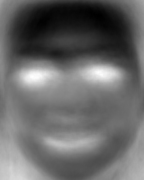
\includegraphics[width=0.1\textwidth]{images/eigenfaces/eigenface00} & 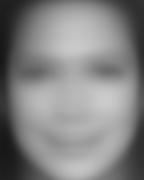
\includegraphics[width=0.1\textwidth]{images/eigenfaces/eigenface01} &
		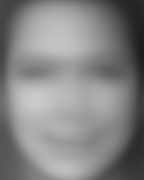
\includegraphics[width=0.1\textwidth]{images/eigenfaces/eigenface02} & 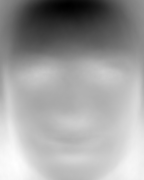
\includegraphics[width=0.1\textwidth]{images/eigenfaces/eigenface03} &
		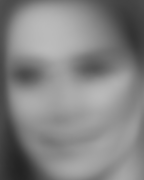
\includegraphics[width=0.1\textwidth]{images/eigenfaces/eigenface04} &
		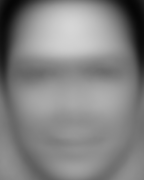
\includegraphics[width=0.1\textwidth]{images/eigenfaces/eigenface05} & 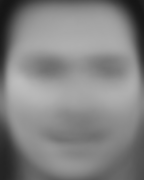
\includegraphics[width=0.1\textwidth]{images/eigenfaces/eigenface06} &
		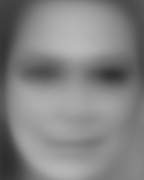
\includegraphics[width=0.1\textwidth]{images/eigenfaces/eigenface07} \\ 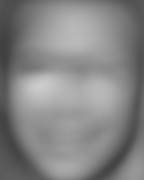
\includegraphics[width=0.1\textwidth]{images/eigenfaces/eigenface08} &
		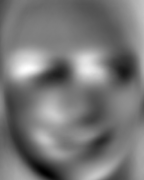
\includegraphics[width=0.1\textwidth]{images/eigenfaces/eigenface09} & 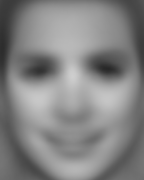
\includegraphics[width=0.1\textwidth]{images/eigenfaces/eigenface10} &
		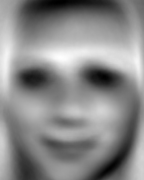
\includegraphics[width=0.1\textwidth]{images/eigenfaces/eigenface11} & 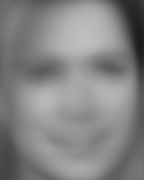
\includegraphics[width=0.1\textwidth]{images/eigenfaces/eigenface12} &
		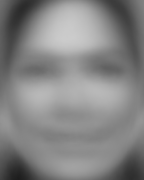
\includegraphics[width=0.1\textwidth]{images/eigenfaces/eigenface13} & 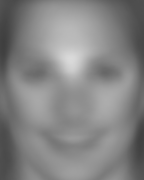
\includegraphics[width=0.1\textwidth]{images/eigenfaces/eigenface14} &
		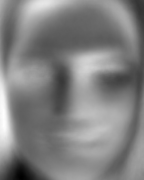
\includegraphics[width=0.1\textwidth]{images/eigenfaces/eigenface15} \\
	\end{tabular}
	\caption{Die ersten 16 Eigengesichter wurden wieder als Bild dargestellt.}
	\label{fig:eigenfaces}
\end{figure}

Im Grunde fangen die Eigengesichter charakteristische Gesichtszüge ein.
Mit charakteristisch ist hier gemeint, dass genau diese Gesichtszüge für die grösste Varianz\footnote{Das Wort \glqq{}Varianz\grqq{} kommt aus der Statistik und hat eine formale Definition. Für uns ist aber nur wichtig, dass sie ein Mass für die Streuung von Daten (in diesem Fall Gesichter) ist.} unter allen Bildern der Datenbank verantwortlich sind.
Sie beschreiben die Merkmale, nach denen sich die Gesichter am meisten unterscheiden.
Besser gesagt: Das erste Eigengesicht fängt den Gesichtszug mit der grössten Varianz ein.
Die weiteren Eigengesichter fangen Gesichtszüge mit immer weniger Varianz ein.
Dies spiegelt sich auch in deren Konstruktion wieder, welche die Eigengesichter ja gerade als Vektoren entlang der grössten Streuung definiert.